% !TEX root = ../Seminararbeit-Data_Mining_Frameworks.tex
%


% =============================================================================
%
% Fazit
%
% =============================================================================
\chapter{Fazit}
\label{sec:fazit}

Zum Abschluss werden beide Tools noch einmal in Bezug auf unterschiedliche
Aspekte miteinander verglichen.

\begin{enumerate}
  \item Installation und Setup: \\
  Zunächst konnte das „Setup“ bei beiden Tools ohne Probleme durchgeführt
  werden. Allerdings besitzt das Microsoft Azure Machine Learning Studio
  hier den Vorteil, dass keine Installation (sondern nur eine Registrierung
  bzw. ein Login) notwendig ist und man direkt mit der Analyse seiner Daten
  beginnen kann. Das RapidMiner Studio ist zwar für alle Plattformen erhältlich,
  muss aber dennoch (manuell) installiert werden. Zudem wird eine aktuelle Java
  Runtime vorausgesetzt, welche u.U. auch erst installiert werden muss.
  Microsoft setzt diesbezüglich nur einen (aktuelleren) Internetbrowser voraus.
  \item Features und Funktionen: \\
  Beide Programme kommen mit einer Vielzahl an Implementierungen verschiedener
  Algorithmen. Bezüglich der Anzahl hat das RapidMiner Studio jedoch etwas mehr
  zu bieten.


  \begin{figure}[htb]
    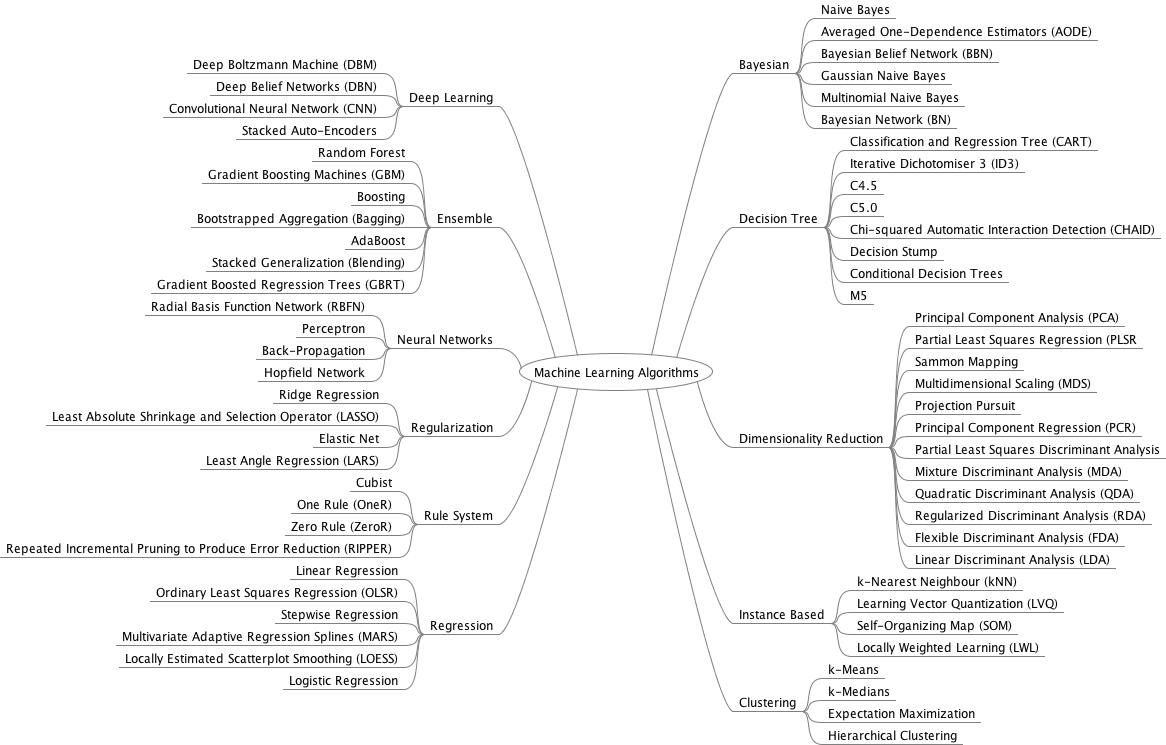
\includegraphics[width=\textwidth]{gfx/rmalgs.png}
    \caption{Algorithmen des RapidMiner Studios \cite{MLM}}
    \label{fig:fazit:rmalgs}
  \end{figure}

  \begin{figure}[htb]
    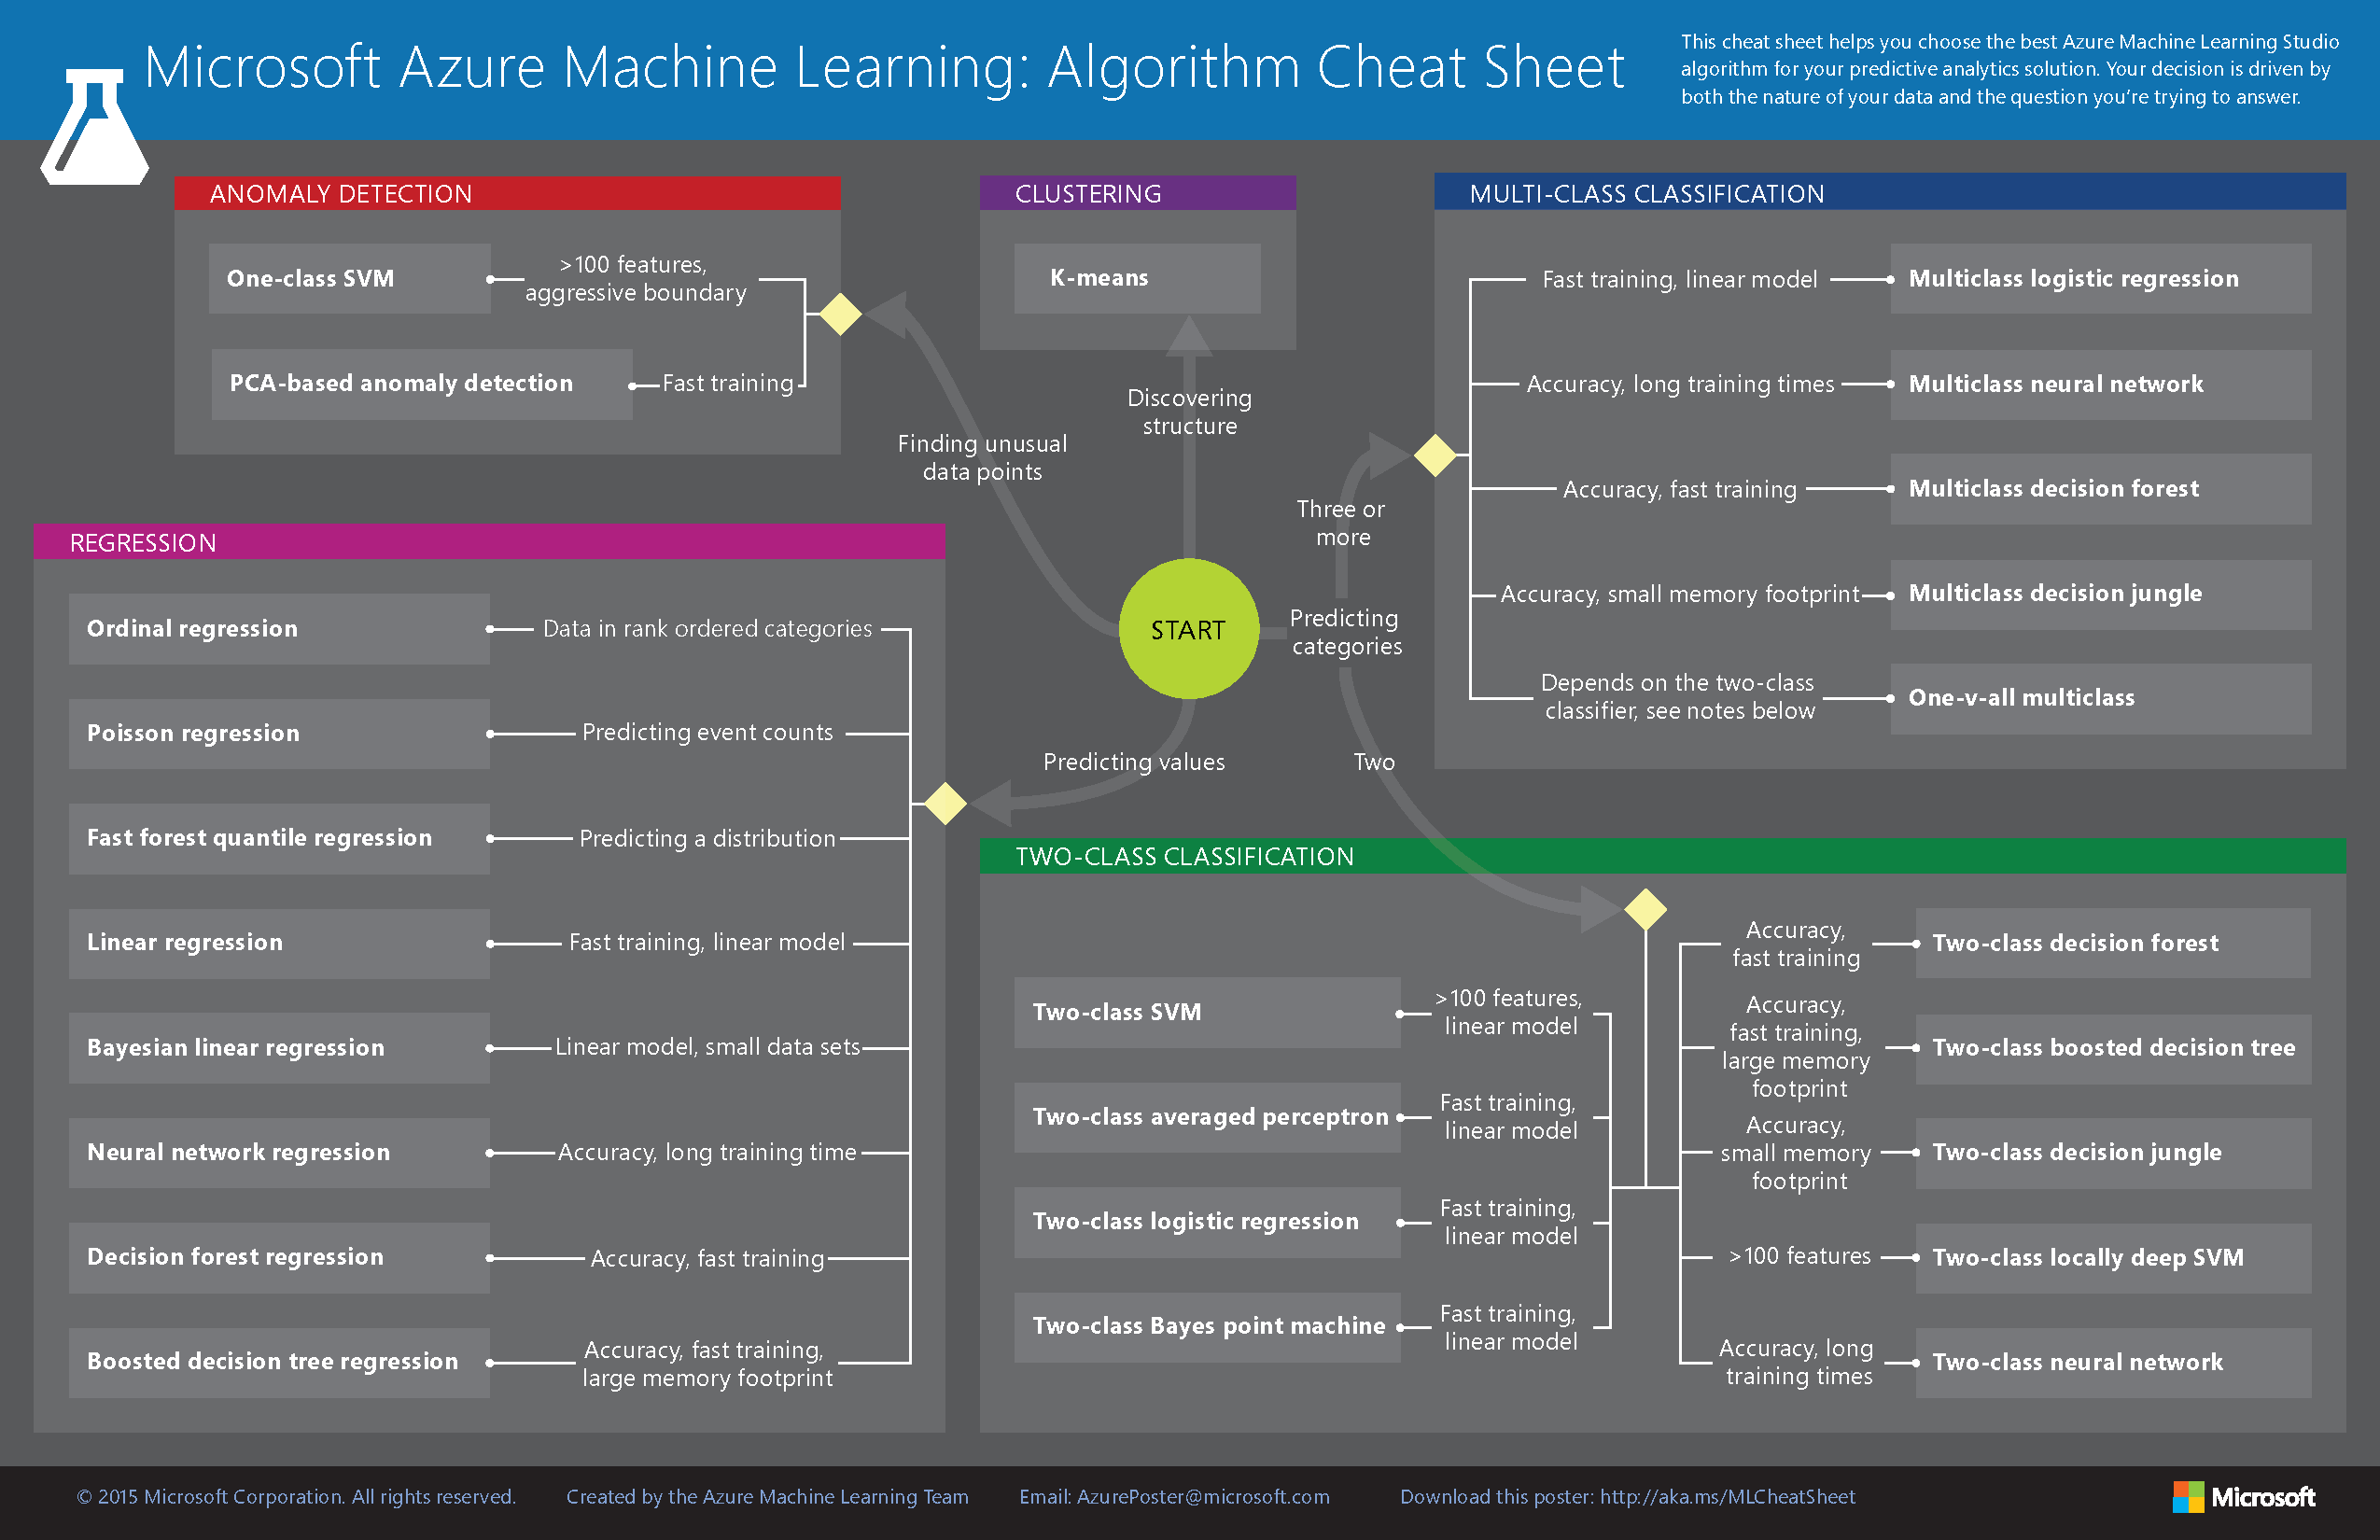
\includegraphics[width=\textwidth]{gfx/msaalgs.pdf}
    \caption{Algorithmen des Microsoft Azure Machine Learning Studios \cite{MSA}}
    \label{fig:fazit:msaalgs}
  \end{figure}
  \item Kollaboration und Zusammenarbeit:
 \\
  Gleiches wie bei der Automatisierung gilt auch für die Unterstützung eines
  kollaborativen Workflows mit mehreren Anwendern. Während in Microsofts
  Machine Learning Studio die Experimente direkt mit anderen Anwendern geteilt
  bzw. zusammen an diesen gearbeitet werden kann, benötigt es auf der RapidMiner
  Plattform eines eigenen Servertools (sofern die Prozesse nicht als Datei
  abgespeichert und per Email verschickt werden wollen).
  \item Bedienung und User Interface: \\
  Bezüglich der Bedienbarkeit bietet das RapidMiner Studio einen angenehm hohen
  Komfort, während das Machine Learning Studio von Microsoft an die
  Webtechnologien und Möglichkeiten eines Internetbrowser gebunden ist. Nichtsdestotrotz
  ist die nötige Einarbeitungszeit bei beiden Tools sehr kurz.
  \item Schnittstellen und Erweiterungsmöglichkeiten: \\
  Da das RapidMiner Studio quelloffen ist, ist es hier möglich, durch Plugins
  die Feature-Liste selbst noch zu erweitern und eigene Algorithmen zu
  implementieren. Jedoch bietet das Microsoft Azure Machine Learning Studio
  hier einen deutlich höheren Komfort, indem es direkt das Einbinden von R
  Skripten, sowie Python Code ermöglicht.
  \item Automatisierung und Deployment
: \\
  Die Experimente können aus dem Machine Learning Studio direkt als
  Webservices exportiert und per REST-API angesteuert werden. Dies ermöglicht
  einen sehr effizienten und schnellen Workflow von der Analyse der Daten hin
  zur Implementierung eines automatisierten Modells in einer bestehenden
  Anwendung. RapidMiner Studio benötigt dagegen für das Deployment einen
  eigene Serverinstallation auf Basis des RapidMiner Servers oder des RapidMiner
  Radoop Tools. Der Administrationsaufwand ist hier daher deutlich höher.
\end{enumerate}

Abschließend lässt sich sagen, dass RapidMiner zurecht die populärere der
beiden Plattformen ist, da diese intuitiver zu bedienen ist und in Sachen
vorgefertigter Algorithmen deutlich mächtiger ist als die Lösung von Microsoft.
Nichtsdestotrotz sollte auch, gerade wenn bereits ein Informationssystem auf
Basis von Microsoft bzw. der Azure Cloud besteht, das Machine Learning Studio
nicht außer Acht gelassen werden.
